\documentclass[tikz,border=3.14mm]{standalone}
\usepackage{pgfplots}
\pgfplotsset{compat=1.16}
\begin{document}
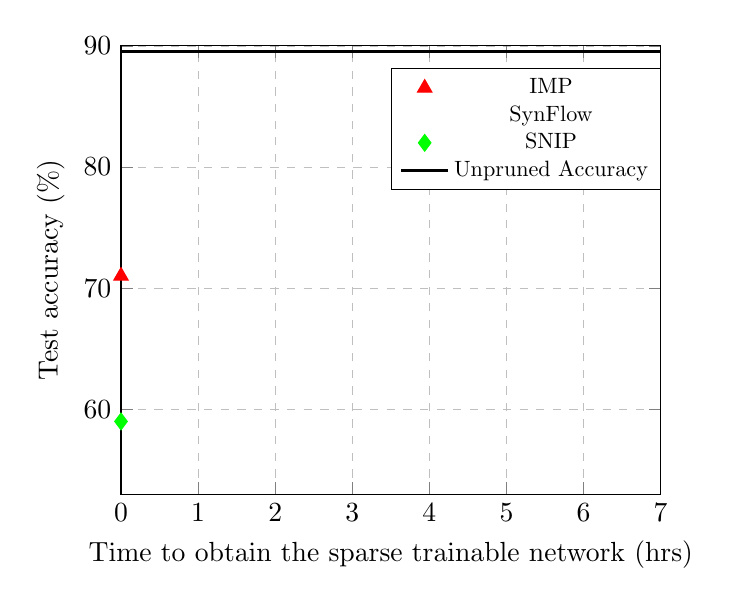
\begin{tikzpicture}
\begin{axis}[
    xlabel={Time to obtain the sparse trainable network (hrs)},
    ylabel={Test accuracy (\%)},
    xmin=0, xmax=7,
    ymin=53, ymax=90,
    legend style={at={(0.5,0.95)},anchor=north west,nodes={scale=0.8, transform shape}},
    grid=both,
    grid style={line width=.1pt, dashed},
    major grid style={line width=.2pt,dashed}
]
\addplot[
    only marks,
    mark=triangle*,
    mark size=3pt,
    color=red
]
coordinates {
    (0,71)
};
\addlegendentry{IMP}

\addplot[
    only marks,
    mark=circle*,
    mark size=3pt,
    color=blue
]
coordinates {
    (0,74)
};
\addlegendentry{SynFlow}

\addplot[
    only marks,
    mark=diamond*,
    mark size=3pt,
    color=green
]
coordinates {
    (0,59)
};
\addlegendentry{SNIP}

\addplot[
    color=black,
    line width=1pt
]
coordinates {
    (0,89.5)(7,89.5)
};
\addlegendentry{Unpruned Accuracy}
\end{axis}
\end{tikzpicture}
\end{document}